\documentclass{article}

\usepackage{fullpage} 
\usepackage[doublespacing]{setspace}
\usepackage{amsmath, amssymb,amsfonts} 
\usepackage[small]{caption}
\usepackage{graphicx} 
\usepackage{float} 
\usepackage{subfig}
\usepackage{xspace} 
\usepackage{natbib}
\usepackage{datetime} %provides \currenttime command

\graphicspath{{./Figures/}} \DeclareGraphicsExtensions{.pdf, .jpg, .png}

%BCO: Look at what Science recommends for manuscripts using LaTeX
%(they clearly want to say "go away" but can't):
%http://www.sciencemag.org/site/feature/contribinfo/prep/TeX_help/tex2pdf.xhtml


%%%%%%%%%%%%%%%%%%%%%%%%%%%%%%%%%Local Commands%%%%%%%%%%%%%%%%%%%%%%%%%%%%%
%%% Sort using M-x 'sort-lines'
\newcommand{\Costaobsvec}{\ensuremath{\Cost(\aobsvec)}\xspace}
\newcommand{\Costaveci}{\ensuremath{\Cost(\aveci)}\xspace}
\newcommand{\Costavecj}{\ensuremath{\Cost(\avecj)}\xspace}
\newcommand{\Costavec}{\ensuremath{\Cost(\avec)}\xspace}
\newcommand{\Costcveci}{\ensuremath{\Cost(\cveci)}\xspace}
\newcommand{\Costcvecj}{\ensuremath{\Cost(\cvecj)}\xspace}
\newcommand{\Cost}{\ensuremath{\text{\textbf{Cost}}}\xspace}
\newcommand{\DeltaAIC}{\ensuremath{\Delta\text{AIC}}\xspace}
\newcommand{\EE}{\mathbb{E}} %use for expectation function E()
\newcommand{\Funcaobsvec}{\ensuremath{\Func(\aobsvec|\aoptvec)}\xspace}
\newcommand{\Funcaoptvec}{\ensuremath{\Func(\aoptvec)}\xspace}
\newcommand{\Funcaveci}{\ensuremath{\Func(\aveci|\aoptvec)}\xspace}
\newcommand{\Funcavecj}{\ensuremath{\Func(\avecj|\aoptvec)}\xspace}
\newcommand{\Funcavec}{\ensuremath{\Func(\avec|\aoptvec)}\xspace}
\newcommand{\Funccveci}{\ensuremath{\Func(\cveci|\aoptvec)}\xspace}
\newcommand{\Funccvec}{\ensuremath{\Func(\cvec|\aoptvec)}\xspace}
\newcommand{\Func}{\ensuremath{\text{\textbf{Benefit}}}\xspace}
\newcommand{\GTR}{GTR+$\Gamma$\xspace}
\newcommand{\LogN}{\ensuremath{\text{LogN}}\xspace}
\newcommand{\Ne}{\ensuremath{{N_e}}\xspace} %
\newcommand{\Nemu}{\ensuremath{{N_e \mu}}\xspace} %
\newcommand{\Piihat}{\ensuremath{\hat{\pi}_i}\xspace}
\newcommand{\Pii}{\ensuremath{\pi_{i}}\xspace}
\newcommand{\Pijhat}{\ensuremath{\hat{\pi}_j}\xspace}
\newcommand{\Pij}{\ensuremath{\pi_{j}}\xspace}
\newcommand{\Pivechat}{\ensuremath{\hat{\Pivec}}\xspace}
\newcommand{\Pivec}{\ensuremath{\Vec{\pi}}\xspace}
\newcommand{\Qmatrixa}{\ensuremath{\Qmatrix_a}\xspace}
\newcommand{\Qmatrix}{\mathbf{Q}\xspace}
\newcommand{\Wi}{\ensuremath{{W_i}}\xspace}
\newcommand{\Wj}{\ensuremath{{W_j}}\xspace}

\newcommand{\acivec}{\ensuremath{a\left(\cveci\right)}\xspace}
\newcommand{\acvecg}{\ensuremath{a\left(\vec{c}_{i,g}\right)}\xspace}
\newcommand{\acvecj}{\ensuremath{a\left(\cvecj\right)}\xspace}
\newcommand{\acvec}{\ensuremath{a\left(\Vec{c}\right)}\xspace}
\newcommand{\aip}{\ensuremath{a_{i,p}}\xspace}
\newcommand{\aivecg}{\ensuremath{{\avec}_{i,g}}\xspace}
\newcommand{\aivec}{\aveci}
\newcommand{\ajp}{\ensuremath{a_{j,p}}\xspace}
\newcommand{\ajvecg}{\ensuremath{{\ajvec}_{,g}}\xspace}
\newcommand{\ajvec}{\ensuremath{\Vec{a}_{j}}\xspace}
\newcommand{\aj}{\ensuremath{a__j}\xspace}
\newcommand{\alphac}{\ensuremath{\alpha_c}\xspace}
\newcommand{\alphag}{\ensuremath{\alpha_G}\xspace}
\newcommand{\alphap}{\ensuremath{\alpha_p}\xspace}
\newcommand{\alphavec}{\ensuremath{\Vec{\alpha}}\xspace}
\newcommand{\alphav}{\ensuremath{\alpha_v}\xspace}
\newcommand{\alphavValue}{\ensuremath{4 \times 10^{-4}}\xspace}
\newcommand{\aobsvecg}{\ensuremath{{\avec}_{\text{obs},g}}\xspace}
\newcommand{\aobsvec}{\ensuremath{\Vec{a}_{\text{obs}}}\xspace}
\newcommand{\aobs}{\ensuremath{a_{\text{obs}}}\xspace}
\newcommand{\aopt}{\ensuremath{a_*}\xspace}
\newcommand{\aoptip}{\ensuremath{\aopt_{i,p}}\xspace}
\newcommand{\aoptpg}{\ensuremath{\aopt_{p,g}}\xspace}
\newcommand{\aoptp}{\ensuremath{a_{*,p}}\xspace}
\newcommand{\aoptvecg}{\ensuremath{{{\aoptvec}_g}}\xspace}
\newcommand{\aoptvec}{\ensuremath{\Vec{a}_*}\xspace}
\newcommand{\aveci}{\ensuremath{\Vec{a}_i}\xspace}
\newcommand{\avecj}{\ensuremath{\Vec{a}_j}\xspace}
\newcommand{\avec}{\ensuremath{\Vec{a}}\xspace}
\newcommand{\cveci}{\ensuremath{\cvec_i}\xspace}
\newcommand{\cvecj}{\ensuremath{\cvec_j}\xspace}
\newcommand{\cvec}{\ensuremath{\Vec{c}}\xspace}
\newcommand{\deltaT}{\ensuremath{\delta t}\xspace}
\newcommand{\etag}{\ensuremath{\eta_g}\xspace}
\newcommand{\fij}{\ensuremath{f_{i,j}}\xspace}
\newcommand{\jmax}{\ensuremath{{j_{\max}}}\xspace}
\newcommand{\kmax}{\ensuremath{{k_{\max}}}\xspace}
\newcommand{\muij}{\ensuremath{\mu_{i,j}}\xspace}
\newcommand{\phig}{\ensuremath{\phi_{g}}\xspace}
\newcommand{\pij}{\ensuremath{p_{i,j}}\xspace}
\newcommand{\qij}{\ensuremath{q_{i,j}}\xspace}
\newcommand{\qji}{\ensuremath{q_{i,j}}\xspace}
\newcommand{\setG}{\ensuremath{\mathbb{G}}\xspace}
\newcommand{\setP}{\ensuremath{\mathbb{P}}\xspace}
\renewcommand{\ng}{\ensuremath{{n_g}}\xspace}
\newcommand{\gp}{\ensuremath{{G_p}}\xspace}
\DeclareMathOperator{\Var}{Var}

\title{Population genetics models with selection for phylogenetic
inference} \date{Last compiled on \today\xspace at \currenttime.}
\begin{document}
\maketitle


\section*{Abstract}
We present a phylogenetic approach rooted in the field of population genetics that more realistic models the evolution of protein-coding DNA under the assumption of stabilizing selection.
The new set of models, which we collectively call selac models, fit phylogenetic data substantially better than current models, suggesting more accurate inference of phylogenies.
Moreover, these models allow inference of population genetics parameters from data used for interspecific phylogenies.

\section*{Introduction}
Phylogenetic analysis now plays a critical role in the fields of ecology, evolution, paleontology, medicine, conservation, and others.
While the scale and impact of phylogenetic studies has increased substantially over the past two decades, the realism of the models used to infer the trees has changed relatively little by comparison.
The simplest models assume neutrality between the different amino acid substitutions and may or may not include mutation bias (e.g.~F81, F84, HYK85, TN93, and GTR for the former and JC69 and K80 for the latter, see \citet{Yang2014} for an overview).
The next set of models attempt to include a 'selection' term $\omega$ which is interpreted as describing stabilizing or diversifying selection depending on whether $\omega$ is less than or greater than 1, respectively. 
%frequency dependent selection or over- or underdominance
However, the link between $\omega$ and the key parameters found in standard population genetics models of Wright and Fisher or Moran, such as \Ne, the distribution of $s$ across genotype space, and mutation bias are far from clear andl likely only describe a subset of scenarios such as over/underdominance or frequency dependent selection  \citep{HughesAndNei1988}.
Fortunately, given the continual growth in computational power available to researchers, it is now possible to utilize a more general set of population genetics based models for the purpose of phylogenetic reconstruction \citep[e.g.][]{HalpernAndBruno1998,RobinsonEtAl2003,LartillotAndPhilippe2004,RodrigueAndLartillot2014}.

The field of population genetics is a mature, mathematically rigorous, and well established framework for describing biological evolution.
Despite the fact that there are only a few fundamental evolutionary forces at play, i.e.~mutation, drift, selection, and linkage effects, describing the evolutionary behavior of a system in which there are non-linear interactions between different sites quickly becomes overwhelmingly complex.
In contrast, under the simplifying assumptions of additivity between and within sites, calculating stationary and substitution probabilities are relatively straightforward to calculate.
As a result, fitting additive models of the evolutionary process to sequence data is computationally feasible.
One major advantage to fitting models derived from population genetics over other approches is that the parameters estimated are biologically meaningful and of great interest to evolutionary biologists.
For example in haploid population, if the product of effective population size $\Ne$ and the mutation rate of beneficial alleles $\mu_b$ is greater than one, then the waiting time for an adaptive allele to emerge after an environmental shift is much shorter than the substitution process itself and evolution itself is not mutation limited.
Here we show how fitting a phylogenetic model derived from a population genetic model can be used to estimate $\Nemu$ as well as the optimal amino acid sequence of a protein and the average protein synthesis rate of each gene using only coding sequence data from the tips of the tree.

The model we develop can be viewed as a special formulation of the Wright-Fisher (WF) model \citep{Kimura1962,Wright1969,Iwasa1988,BergAndLassig2003,SellaAndHirsh2005}.
We ignore linkage effects and, as a result of this and other assumptions, our model behaves in a site independent manner.
Our approach is developed in the same vein as previous phylogenetic applications of the WF model \citep[e.g.][]{MuseAndGaut1994,HalpernAndBruno1998,YangAndNielsen2008,RodrigueEtAl2005,KoshiAndGoldstein1997,KoshiEtAl1999,DimmicEtAl2000,ThorneEtAl2012,LartillotAndPhilippe2004,RodrigueAndLartillot2014}. % and other contexts \citep{WilkeAndDrummond2006,Gilchrist2007,DrummondAndWilke2009,GilchristEtAl2015}.\footnote{mikeg: When and how often to refer to our model as `MutSel' ala YN08 and Wilke.}
Similar to \citet{LartillotAndPhilippe2004,RodrigueAndLartillot2014} we assume there is a finite set of rate matrices describing the substitution process and that each position within a protein must assigned to a particular rate matrix category.%\footnote{mikeg: If this is too detailed for the intro, this paragraph could be moved to the Discussion and summarized more succinctly here.}
Unlike othe researchers, we assume \emph{a priori} there are 20 different families of rate matrices, one family for when a given amino acid is favored at a site.
As a result, our approach allows us to quantiatively evaluate the support for a particular amino acid being favored over all the 19 other at a particular position within the protein encoded by a particular gene.
% category corresponds to identifying which amino acid is favored over the others for a given site (i.e.~optimal at that position within the protein).

Because our approach requires twenty families of $20 \times 20$ matrices, the number of parameters needed to implement our model would, without further simplification, be extremely large.
To reduce the number of parameters needed while still maintaining a high degree of biological realism, we construct our gene and amino acid specific substitution matrices using a submodel.
As a result, our model requires only a handful of parameters that are used genome wide such as nucleotide specific mutation parameters, the effective population size \Ne, and side chain physiochemical weighting parameters.
In addition to these genome wide parameters, our model requires two gene specific parameters: an expression parameter, $\phi$ which scale the average strength of stabilizing selection for the optimal amino acid at each position and a variance parameter which describes how the strength of stabilizing selection varies around the mean value between positions.
Because we use a submodel to derive our substitution matrices, our model requires the estimation of a fraction of the parameters required when compared to approaches where the substitution rates are allowed to vary independently  \citep{HalpernAndBruno1998,LartillotAndPhilippe2004,RodrigueAndLartillot2014}.


The work we present here contributes to the field of phylogenetics and molecular evolution in a number of ways.
Our model provides an complementary example to \citet{ThorneEtAl2012} studies of how models of molecular and evolutionary scales can be combined together in a nested manner.
Our use of model nesting also allows us to formulate and test specific biological hypotheses.
For example, we are able to compare a model formulation which assumes that physio-chemical deviations from the optimal sequence are equally disruptive at all sites within a protein to one which assumes they vary between sites.
We've utilized the same nested, population genetic based approach in more traditional genomic analyses \citep[e.g.][]{Gilchrist2007,ShahAndGilchrist2011,GilchristEtAl2015}.
That work and our current work illustrates how more information can be extracted from sequence data when more biologically based models are used.
While the mapping between genotype and phenotype is more abstract than \citet{ThorneEtAl2012}, our approach has the advantage of not requiring a model of a protein's physical structure.
By linking the strength of stabilizing selection to gene expression, specifically the average synthesis rate of a protein, we can weight the historical information encoded in different genes in a biologically defensible manner while simultaneously estimating their expression levels.




\section*{Results}
\subsection*{Model Performance}

\begin{enumerate}
\item Using \DeltaAIC as our measure, we see that even despite the need for estimating the optimal amino acid at each position in each protein, our model performs astronomically better than GTR, GY94, or YN08.
\item Including the random effects term $G$ not only provides greater biological realism than assuming $G =1$, it provides substantially better model fit.
\newcommand{\subfigwidth}{0.4\textwidth}
\begin{figure}[H]
  \centering
  \subfloat[\ ]{\frame{\includegraphics[width=\subfigwidth]{yeast_SELACgamma.pdf}}}
  \qquad
  \subfloat[\ ]{\frame{\includegraphics[width=\subfigwidth]{yeast_SELACnogamma.pdf}}}
  \qquad
  \subfloat[\ ]{\frame{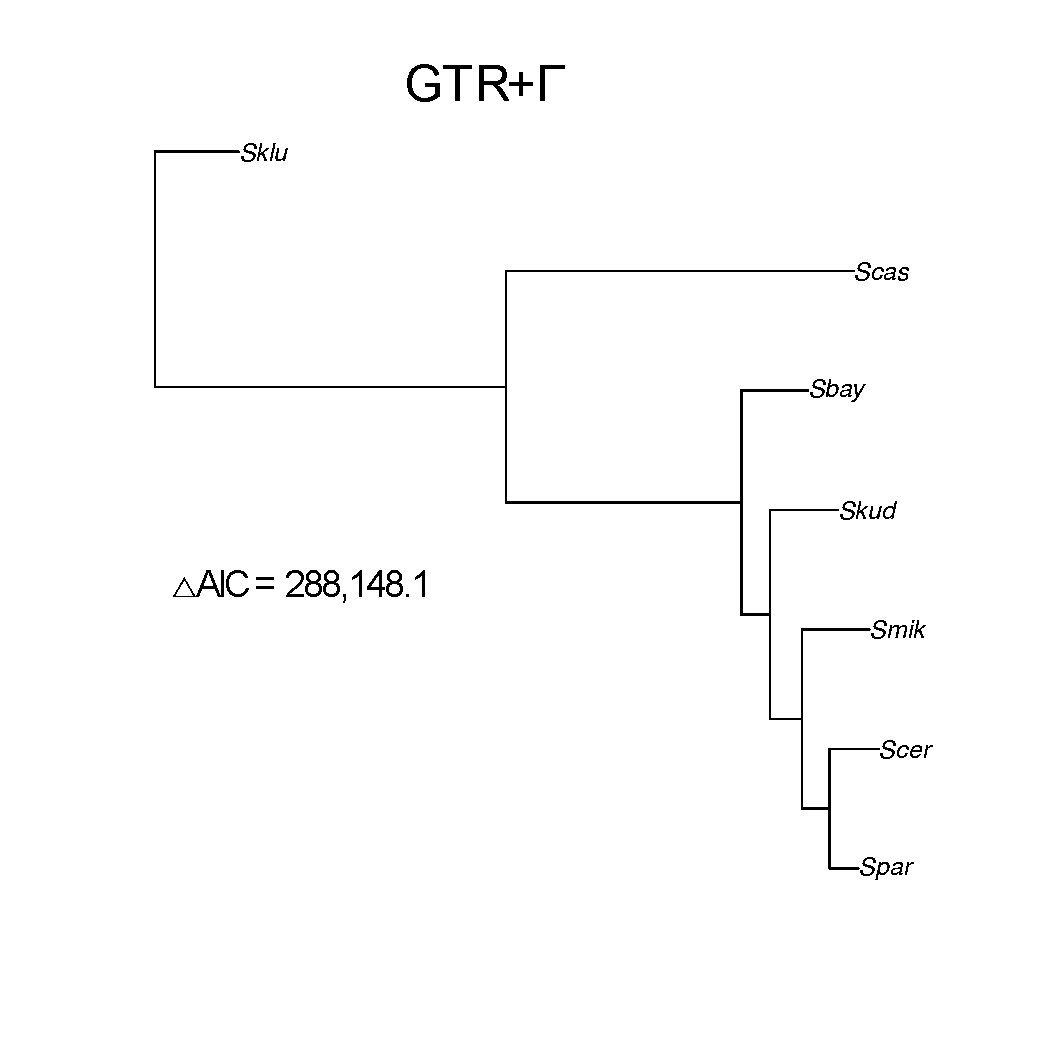
\includegraphics[width=\subfigwidth]{yeast_GTR.pdf}}}
  \qquad
  \subfloat[\ ]{\frame{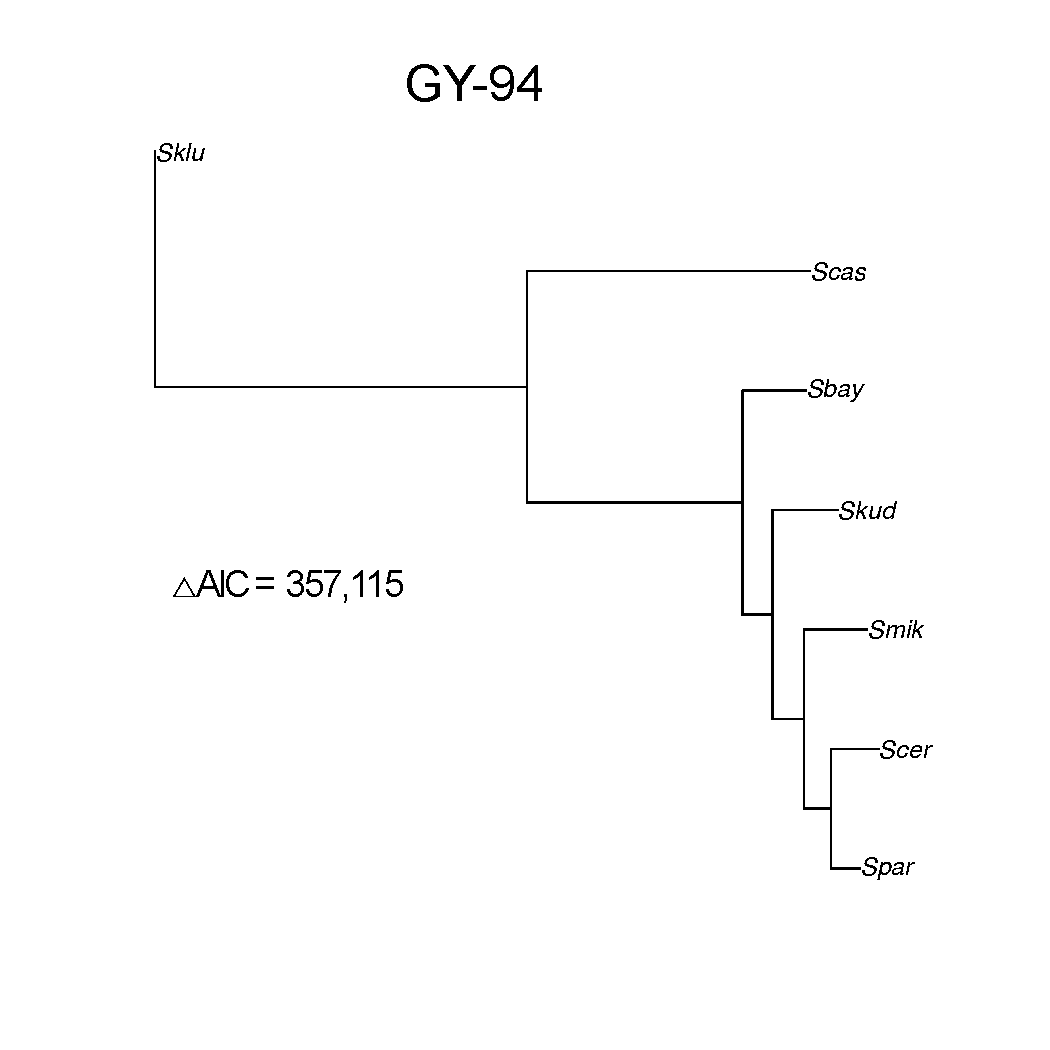
\includegraphics[width=\subfigwidth]{yeast_GY94.pdf}}}
  \qquad
  \subfloat[\ ]{\frame{\includegraphics[width=\subfigwidth]{yeast_YN2008.pdf}}}
  \qquad
  \subfloat[\ ]{\frame{\includegraphics[width=\subfigwidth]{yeast_LGY2004.pdf}}}
  \caption{Maximum Likelihood Trees for (a) selac, (b) selac with uniform sensitivity $G = 1$, (c) GTR, (d) GY94, and (e) YN08, (f) \citet{LartillotAndPhilippe2004}.}
  \label{fig:MleTrees}
\end{figure}
\item Table of number of parameters, estimates for key parameters (or their summaries), and \DeltaAIC values.
\item The gene specific estimate of \alphag provides an estimate of the variance in sensitivity across sites where $\Var(G) = 1/\alphag$.  
\item Selac provides estimates of gene expression which are positively correlated with empirical estimates and explain about 7\% of the variation in the empirical measurements taken during log growth phase.\footnote{mikeg: We should replace the estimates of $\phi$ with estimates of $\psi$ which is $\phi/\Funcaobsvec$} 

\renewcommand{\subfigwidth}{0.4\textwidth}
\begin{figure}[H]
  \centering
  \subfloat[\ ]{\frame{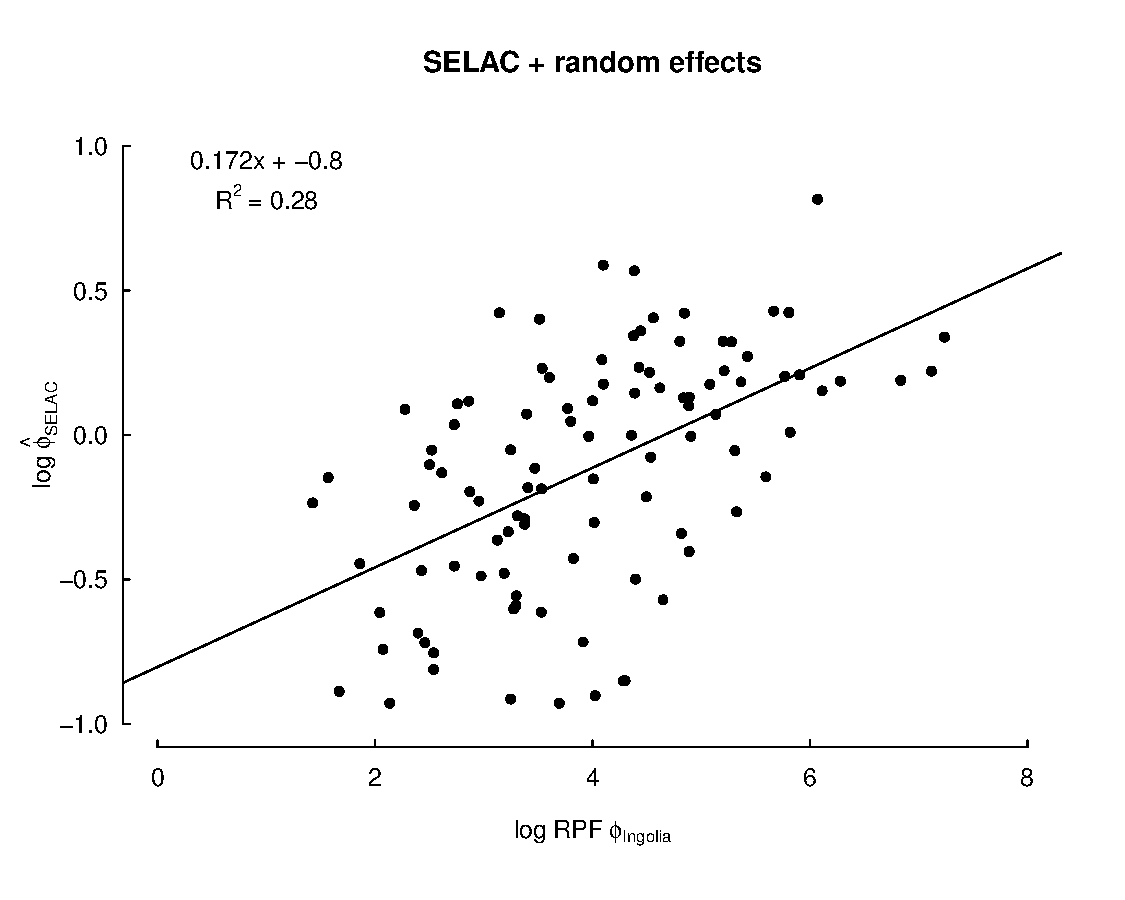
\includegraphics[width=\subfigwidth]{RPF_vs_Phi/RNA_abunIngolia_vs_SelACphiGamma}}}
  \qquad
  \subfloat[\ ]{\frame{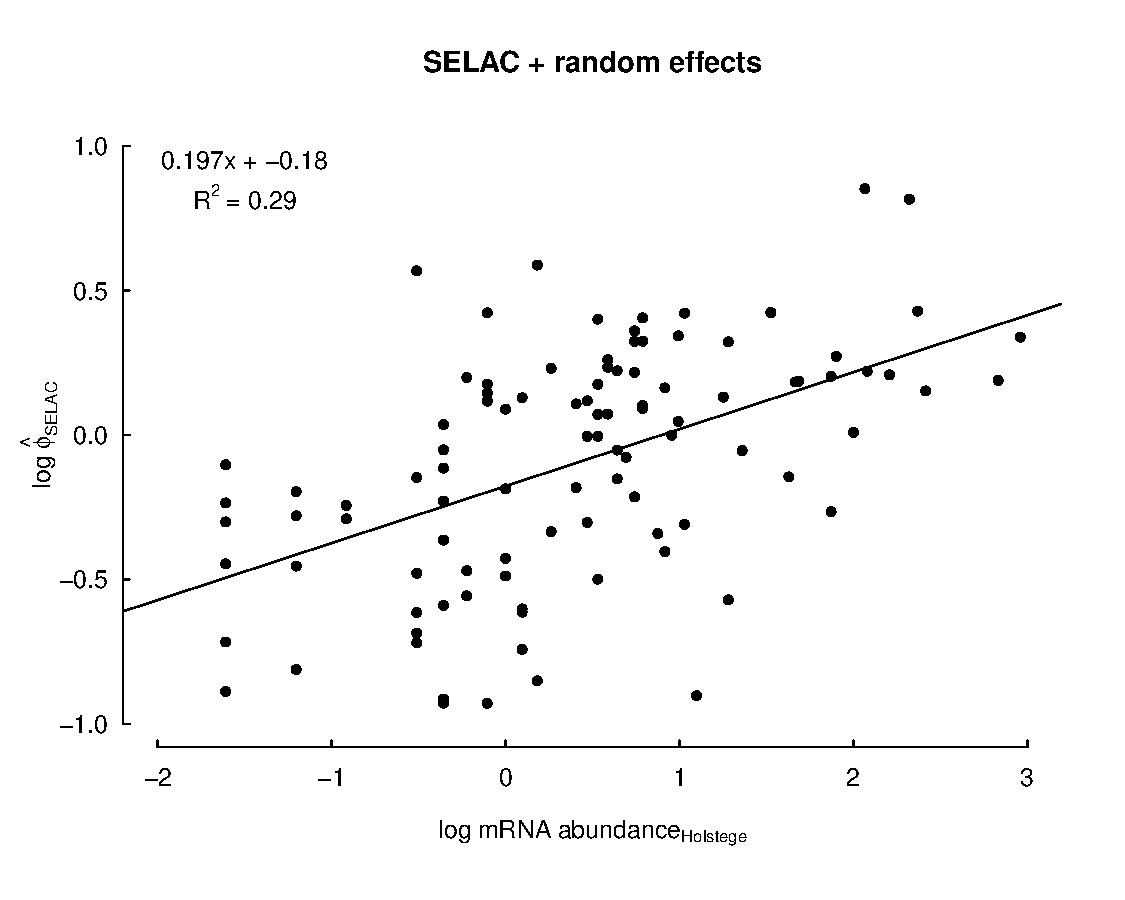
\includegraphics[width=\subfigwidth]{mRNA_vs_Phi/mRNA_abunHolstege_vs_SelACphiGamma}}}
\caption{Comparison of log protein synthesis rate $\phi$  estimated by selac and (a) estimates from ribosome profile footprint data of \citet{IngoliaEtAl2009} and \citet{HolstegeEtAl1998}.
}
\end{figure}
\item By linking $q$ to gene expression, our approach is an alternative to the more common approach of simply concatenation of protein coding sequences.
More specifically, in our model simply concatenating gene sequences together is equivalent to assuming the same aver protein synthesis rate $\phi$ for all of the genes.
By assuming the strength of stabilizing selection for the optimal sequence, \aoptvec, is proportional to $\phi$, our model allows us to estimate $\phi$ for each gene.
Our results clearly indicate that this information is available and accounting for it in our model substantially improves our model fit.
\item [Lots of other stuff]
\end{enumerate}
\section*{Discussion}

\begin{itemize}
\item One important manner in which our approach moves beyond \citet{HalpernAndBruno1998,RobinsonEtAl2003,LartillotAndPhilippe2004,ThorneEtAl2012,RodrigueAndLartillot2014} is in that we parameterize the model and fit branch lengths simultaneously rather than in two separate steps.\footnote{mikeg: Jeremy or Brian: I know this is true for Halpern and Bruno and am 95\% sure it applies to Jeff Thorne's work.
Can you confirm its true for the Lartillot references?}
\item Assumptions of additivity and no epistasis are unrealistic but can be viewed as a first order approximation to these more complex scenarios and a starting point for later relaxing these assumptions.
\item Implicitly, our model assumes that all genes are essential because an organism that is homozygous for alleles with zero activity (i.e.~no benefit) would have to spend an infinite amount of energy to achive a target functionality production rate $\phi > 0$.
This assumption can be relaxed by allowing $\phi$ to vary and fitness is function of that $\phi$ level and where there is an optimal $\phi$ level.
\item Note that our definition of $\phi$ and our scaling of functionality differ slightly from our previous work \citep{Gilchrist2007,GilchristEtAl2009,ShahAndGilchrist2011,GilchristEtAl2015}.
In our previous work, we were concerned with how changes in synonymous codons affected error rates and synthesis costs and, as a result, defined functionality relative to an error free protein, rather than an optimal one, and conflated $\phi$ and $\psi$.
\item Our approach requires relatively few parameter. 
  \begin{enumerate}
  \item Distance function $d(a_i, \aopt)$: If $n_d$ is the number of physiochemical properties examined, the number of parameters estimated is $n_d - 1$
  \item Benefit function $\Func$: If $n_A$ is the order of our Taylor Series approximation, the number of parameters is $n_A-1$.
  \item Gene expression $\phi$: One $\phi$ for each gene analyzed.
  \item Mutation bias: Depends on the model used it is either equal to the number of parameters in the model $n_\mu$ or $n_\mu-1$.
  \end{enumerate}
\item Our approach can be expanded by allowing the optimal amino acid to change during the course of evolution.
This should allow us to use a large, single 400 x 400 matrix instead of 20 separate 20x20 matrices.
The new elements would contain the rates at which the optimal amino acid at site switches from its current state to another amino acid.
Further, if we may be able to compare the statistical properties of this extended transition matrix to the single transition matrix used in other approaches.
\item We conjecture the stationary properties of the 400x400 matrix mentioned above should map to an expected 20 x 20 empirical matrix where we average across when each of the different amino acid are optimal.
\item Statistical Physics model allows decoupling of \Ne, $\mu$, and strength selection.
\end{itemize}


\section*{Additional Points That Need to Be Mentioned}
\begin{itemize}
\item We are measuring and evaluating functional approximation to a more general fitness landscape using sequences at the tip of a tree.
\item In this study we develop a model where the substitution rate of an allele is based on the substitution probability of an allele under selection, mutation bias, and genetic drift, per standard models of population genetics.
\item In developing our model, we assume that for each protein coding gene there is a single amino acid sequence which executes its intended function better than any other sequence, i.e. is optimal.
\item We assume the strength of selection for the optimal sequence increases with the target synthesis rate of the functionality the gene provides.
That is genes with higher target expression levels are under stronger selection than genes with lower target expression levels.
\item We also assume that the functionality of other amino acid sequences declines as the physiochemical properties of the sequence deviates from that of the optimal sequence.
\item We describe how functionality  declines with physiochemical distance using a Taylor series expansion and a set of weighting terms, which we estimate.
\item Because we assume that a protein's functionality is a declining function of the product of the physiochemical distances of each of the protein's amino acid from the optimal, we can treat the evolution at each amino acid position in a site independent manner. 
An approach which is almost universally used in other phylogenetic models.
\item As a result, unlike most phylogenetic approaches, our model requires 20 different 20x20 rate matrices, one for when each amino acid is the optimal one.
\item Even though our model requires a large number of matrices, because of our assumption that a protein's functionality is a declining function of physiochemical distance from the optimum, we are able to parameterize our 20 matrices using only a handful of parameters which we estimate from the data.
\item Two additional key assumption of our model is that (a) the organism has an average target production rate $\phi$ for the functionality provided by each protein and (b) that protein synthesis is under some form of  regulatory control such that the this average functionality production target is met.
As a result, the relative rate of protein synthesis increases as the sequence's functionality declines due to deviation from the optimal sequence.
This behavior, in turn, means that the energetic cost of protein synthesis for an allele deviating from the optimal sequence increases with the target production rate $\phi$.
For example, a protein encoding allele which has a 10\% reduction in functionality will have the same energetic burden and selective cost relative to its optimal sequence as a protein encoding allele of similar length which has a 20\% reduction in functionality but whose target production rate is 1/2 of the first protein.
\item In its current formulation, our model is only applicable to protein coding sequences.
However, it should be applicable to non-coding sequences so long as one has a mapping function between gene sequence and gene function.
\item $\phi$ is determined, in part, by our choice of a reference distance weighting $\alphav = \alphavValue$
\end{itemize}



%BCO: Methods typically go in supplement / end of doc for Science / Nature. So let's plan on that, figuring this will go there. I'm extracting bits to summarize in the main text
\section*{Methods}\label{sec:methods}
The way in which we mathematically link genotype, phenotype, fitness, drift, and fixation, is an extension of a similar approach we have successfully used to study the evolution of codon usage bias using an organisms genome sequence\citep{GilchristAndWagner2006,Gilchrist2007,ShahAndGilchrist2011,GilchristEtAl2015}.
In order to explicitly link the phenotype of genotype to fitness, we assume that organisms have set of fixed but \emph{a priori} unspecified metabolic requirements.
One contribution to meeting these metaboloic requirements met through translation of the proteins encoded in its genome.
We assume that each protein has, on average, a target synthesis rate of $\phi$ and, for now, that $\phi$ is fixed over the tree.
We also assume that natural selection favors genotypes that are able to synthesize their proteome efficiently than their competitors and that each savings of an high energy phosphate bond per unit time leads to a constant proportional gain in fitness $q$.
In terms of the functionality of the protein encoded, we assume that for any given gene there exists an optimal amino acid sequence \aoptvec and that, by definition, a complete, error free peptide consisting of \aopt provides one unit of functionality.
Thus $\phi$ for a given protein is determined by both the organism's metabolic requirements and the functionality of the protein encoded by \aoptvec.
Our approach allows us to link amino acid sequence and gene expression directly to genotype fitness and, in turn, substitution rate in a general, yet simple and biologically plausible, manner.
\footnote{mikeg: Should this stay here?  
  Be parsed down and moved to the intro? 
  Note there is also some redundancy with the text below.}

\subsection*{Allele Substitution Model}
\subsubsection*{Mutation Rate Matrix $\mu$: }
The overall structure of our model involves a codon mutation model combined with a selection model on the codons based on the relative fitness (coming from explicit models of cost and benefits) at a site of the amino acid the codon encodes.
We begin by defining a time reversible model for mutation rates between individual bases.
We use the existing drift driven substitution model JC \citet{JukesAndCantor1969}, also referred to as a General Time Reversible (GTR) \citet{Tavare1986,Yang2014} which has 9 independent parameters, the most possible for a model that assumes mutations occur independently between nucleotides.
This results in a 4x4 mutation matrix, where each entry describes the instantaneous rate of change between a pair of nucleotides for the most recent common ancestor at that site.
This is converted to a $64 \times 64$ codon mutation matrix $\mu$ where entries $\muij$ describe the mutation rate from codon $i$ to $j$ under a 'weak mutation' assumption.
That is, the rate of allele fixation is much greater than \Nemu and $\Nemu \ll 1$, such that evolution is mutation limited, codon substitutions only occur one nucleotide at a time and, as a result,  the rate of change between any pair of codons that differ by more than one nucleotide is zero.
%The above assumptions are commonly made in this field \cite{CITATIONS}\footnote{Do we need to say this?}.

\subsubsection*{Protein Synthesis Cost-Benefit Function $\eta$: }
Our model links fitness to the product of the cost-benefit function of a gene $g$, $\etag$, and the organism's average target production rate of the functionality provided by gene $g$, $\phig$.
This is because the average amount of energy an organism spends to met its target functionality for a gene $g$ is $\etag \times \phig$.
 
\paragraph*{Benefit: }
In order to link genotype to protein function, we first define a benefit function.
This benefit function \Func measures the functionality of the amino acid sequence \aveci encoded by a set of codons \cveci, i.e. $a(\cveci) = \aveci$ relative to that of an optimal sequence $\aoptvec$.
By definition,  $\Funcaoptvec = 1$ and $\Funcaveci < 1$ for all other sequences.
We assume all amino acids within the sequence contribute to protein function and that this contribution declines as an inverse function of physiochemical distance between each amino acid and the optimal.
Formally, we assume that 
\begin{equation}
\Funcaveci = \left(\frac{1}{\ng} \sum_{p=1}^\ng \left(1 + \gp d(\aip, \aoptp\right)\right)^{-1}
\end{equation}
where $\ng$ is the length of the protein, $d(\aip, \aoptp)$ is a weighted physiochemical distance between the amino acid encoded in gene $i$ for position $p$ and $\aoptp$ is the optimal amino acid for that position of the protein.
The term \gp describes the sensitivity of the protein's function to deviation in Grantham's physiochemical space.
We assume that  $\gp \sim \text{Gamma}\left(\alphag, \beta_g = 1/\alphag\right)$ in order to ensure $\EE(\gp) = 1$.
At the limit of $\alphag \rightarrow \infty$, the model collapses to a model with uniform sensitivity of $\gp = 1$ for all positions $p$.
\Funcaveci is an inversely proportional to the average physiochemcial deviation of an amino acid sequence \aveci from the optimal sequence \aoptvec weighted by each sites senstivity to this deviation.
\Funcaveci can be generalized to include second and higher order terms of the distance measure $d$.
%As it stands now, genes can be classified based on their $\alphag$ values.

\paragraph*{Cost}
Generally speaking, protein synthesis involves both direct and indirect assembly costs.
Direct costs consist of the high energy phosphate bonds in ATP or GTP's used to assemble the ribosome on the mRNA, charge tRNA's for elongation, move the ribosome forward along the transcript, and terminate protein synthesis.
Indirect costs are many and consist of the cost of amino acid synthesis as well as synthesis of the protein assembly infrastructure such as ribosomes, aminoacyl-tRNA synthetases, tRNAs, mRNAs, etc.
Direct synthesis costs are the same for all proteins of the same length.
For simplicity, in this study we ignore any indirect costs of protein synthesis that vary between genotypes and define, 
\begin{align}
\label{eq:defineCost}
  \Costcveci  &= \text{Energetic cost of protein synthesis.}\\
  &= C_1 + C_2 n
\end{align}
where, $C_1$ and $C_2$ represent the direct and indirect costs in ATPs of ribosome initiation and peptide elongation, respectively.
When sequence specific costs, such as ribosome pausing times, are included with sequence specific benefits, the probability of a mutant allele fixing is no longer independent of the rest of the sequence.
As a result, our site independent assumption is violated and the fitting of our model becomes much more complex.
For simplicity, in this study we only consider the direct costs of protein assembly and, thus, $C_1 = C_2 = 4  \,\text{ATP}$.\footnote{mikeg: Jeremy, can we let $C_1$ vary as a factor of $C_2$ and then refit the model?}
 



\paragraph*{Defining Physiochemical Distances :}
Assuming that functionality declines with an amino acid $a_i$'s physiochemical distance from the optimum amino acid \aopt at each site  provides a biologically defensible way of mapping genotype to protein function that requires relatively few free parameters.
In addition, our approach naturally lends itself to model selection since we can compare the quality of our model fits using different mixtures of physiochemical properties.
Following \citet{Grantham1974}, we focus on using composition $c$, polarity $p$, and molecular volume $v$ of each amino acid's side chain residue to define our distance function, but emphasize that other properties could be used.
We use the euclidian distance between residue properties where each property $c$, $p$, and $v$ has its own weighting term, $\alphac$, $\alphap$, $\alphav$, respectively.
Because of similar identifiability issues we have with $A_1$ and $\phi$, we set $\alphav = 1$ and recognize that our our estimates of $\alphac$ and $\alphap$ are scaled relative to $\alphav$.
More specifically,
\begin{equation*}
  d(a_i, \aopt) = \sqrt{\alphac \left(c\left(a_i\right) - c\left(\aopt\right)\right)^2 + \alphap \left(p\left(a_i\right) - p\left(\aopt\right)\right)^2 +  \alphav \left(v\left(a_i\right) - v\left(\aopt\right)\right)^2}.
\end{equation*}


\subsubsection*{Linking Cost of Protein Synthesis to Allele Substitution}
In order to link the protein synthesis cost-benefit function $\eta$ of an allele with its fixation probability, we must make a number of assumptions.
First, we assume that each protein encoded within a genome carries out some beneficial function and that the organism needs that functionality to be produced at a target average rate $\phi$.
By definition, the optimal amino acid sequence for a given gene, \aoptvec, produces one unit of functionality.
Second, we assume that protein expression is regulated by the organism to ensure that functionality is produced at rate $\phi$.
As a result, the average protein production rate of a gene, $\psi$, is equal to $\phi/\Func(\avec)$ and the total energy flux allocated towards meeting the target functionality of a particular gene is $\eta(\cvec) \phi$. 
In other words, the cost of a suboptimal protein comes from the need to produce more proteins to get the same overall functionality.


Third, we assume that every additional ATP spent per unit time to meet the organism's target function production rate $\phi$ leads to a slight and proportional decrease in fitness $W$.
This assumption, in turn, implies 
\begin{align}
  W_i\left(\cvec\right) &\propto \exp\left[- q \, \eta(\cveci) \phi\right].
\end{align}
where $q$ describes the decline in fitness with every ATP wasted per unit time used to measure $\phi$ and $\psi$.

Correspondingly, the ratio of fitness between two genotypes is,
\begin{align*}
  W_i/W_j &=  \exp\left[- q \eta(\cveci) \phi\right]/\exp\left[- q \eta(\cvecj) \phi\right]\\
  &=  \exp\left[- q \left(\eta(\cveci)- \eta(\cvecj)\right) \phi\right]\\
\end{align*}
Given our assumptions about $\Nemu$ the \Cost and \Func functions and background mutation rates above, the above fitness ratio for a single position $p$ simplifies to
\begin{align}
 W_i/W_j  &= \exp\left\{- \frac{q}{n} \left(C_1 + C_2 n\right) \left[d\left(\aip,\aoptp\right) - d\left(\ajp,\aoptp\right)\right] \phi \right\}
%Taylor series formulation
%  W_i/W_j &\approx \exp\left[- q \left(C_1 + C_2 n\right) \frac{1}{n}\left(\sum_{p \in \setP} \sum_{k=1}^\kmax A_k \left(d\left(\aip,\aoptp\right)^k - d\left(\ajp,\aoptp\right)^k\right)\right) \phi \right]
%      &=  \exp\left[- q \left(C_1/n + C_2\right)\left(\sum_{p \in \setP} \sum_{k=1}^\kmax A_k \left(d\right(\aip,\aoptp\right)^k - d\left(\ajp,\aoptp\right)^k\right) \phi\right]
\end{align}
where \setP represents the codon positions in which \cveci and \cvecj differ.
Fourth, we make a weak mutation assumption, such that alleles can differ at only one position at any given time, i.e.~$|\setP| = 1$, and that the population is evolving according to a Fisher-Wright process.
As a result, the probability a new mutant $j$ introduced via mutation into a resident population $i$ with effective size \Ne will go to fixation is,
\begin{align*}
  u_{i,j} &=  \frac{1 - \left(W_i/W_j\right)^b}{1 - \left(W_i/W_j\right)^\Ne}\\
%general formulation w/\eta
%   &\approx \frac{1-\exp\left[- q \left(\eta(\cveci)- \eta(\cvecj)\right) \phi b\right]}{1-\exp\left[- q \left(\eta(\cveci)- \eta(\cvecj)\right) \phi 2\Ne\right]}\\
   &= \frac{1- \exp\left\{- \frac{q}{n} \left(C_1 + C_2 n\right) \left[d\left(\aip,\aoptp\right) - d\left(\ajp,\aoptp\right)\right] \phi \,  b\right\}}  {1\exp\left\{- \frac{q}{n} \left(C_1 + C_2 n\right) \left[d\left(\aip,\aoptp\right) - d\left(\ajp,\aoptp\right)\right] \phi \, 2\Ne\right\}}\\
%Taylor series formulation
%   &= \frac{1- \exp\left[- b\,q \left(C_1/n + C_2\right)\left(\sum_{k=1}^\kmax A_k \left(d\right(\aip,\aoptp\right)^k - d\left(\ajp,\aoptp\right)^k\right)\left) \phi\right]}{1-\exp\left[- q \left(C_1/n + C_2\right)\left(\sum_{k=1}^\kmax A_k \left(d\right(\aip,\aoptp\right)^k - d\left(\ajp,\aoptp\right)^k\right)\left) \phi \, 2 \, \Ne\right]},
\end{align*}
where $b=1$ for a diploid population and $2$ for a haploid population \citep{Kimura1962,Wright1969,Iwasa1988,BergAndLassig2003,SellaAndHirsh2005}.
\footnote{mikeg: Jeremy and Brian -- given that the formulation above suggests we can separate out $\phi$ and $\Ne$ when, with the current dataset we cannot.  
Should we use the approximation that can be derived from either \citet{SellaAndHirsh2005} and \citet{Kimura1962} instead?
Alternatively, we could simply discuss this fact and leave the implementation and testing to another day.
}
Finally, assuming a constant mutation rate between alleles $i$ and $j$, $\muij$, where $\muij = 0$ when two codons differ by more than one nucleotide, the transition rate from allele $i$ to $j$ can be modeled as,
\begin{align*}
  q_{i,j} = \frac{2}{b} \muij \Ne u_{i,j}.
\end{align*}
In the end, each optimal amino acid has a separate 64 x 64 substitution rate matrix \Qmatrixa, which incorporates selection for the amino acid (and the fixation rate matrix this creates) as well as the common mutation parameters across optimal amino acids. 
This results in the creation of 20  \Qmatrixa  matrices, one for each amino acid, with up to XXXXX unique rates, based on few parameters (one to six mutation rates, three weights on physiochemical distances, the cost of protein production, target functionality, and optimal amino acid at each site), which we infer from the data.
\footnote{mikeg:  Jeremy previous text included the stop codons and referred to 21 matrices (as it still does below). 
I thought we only modeling only the 20 amino acids.}
Future work will allow transitions between optimal amino acids as well as between codons, which would result in a $(21 x 64) \times (21 x 64) =  1344 \times 1344$ matrix. 


While the overall model does not assume equilibrium, we need still need to scale our substitution matrices $\Qmatrix$.
Traditionally, it is rescaled such that at equilibrium, one unit of branch length represents one expected substitution per site.
In our case, we want to do this scaling across all the matrices, since the branch lengths are used in common across the gene.
One wrinkle is that this must be done taking optimal amino acid frequency into account. 
Here the scaling is done jointly across all the 21 matrices to allow branch lengths under the fixed optimal amino acid model to be comparable to the branch lengths under the global model.
\footnote{mikeg: What do we mean by ``global model''?}
We calculate from the data a vector of 1344 empirical frequencies, $\pi$ for each of the 64 codons observed when assuming each of 21 possible as the optimal amino acid (including stop codons).
A scaling factor is then calculated as the average rate $-\sum_i{} \mu_i*\pi_i=1$, where $i$ indexes a particular codon for a particular optimal amino acid.
The final substitution-rate matrix is the original substitution-rate matrix multiplied by this scaling factor.
This matrix can then be applied to all the sites to calculate the likelihood. 

\subsubsection*{Likelihood Calculations on a Tree: }
Given our assumption of independent evolution among sites, the probability of the whole data set is the product of the probabilities of data at each individual sites.
Thus, the log likelihood is taken as 
\begin{align*}
\text{\textbf{Jeremy: put gamma likelihood equation here?}}
\end{align*}
The log likelihood is maximized by estimating the global parameters: $C \, q \, \Ne$, 9 mutation parameters which are scaled by $2 \Ne/b$, and two Grantham distance parameters, $\alphac$ and $\alphap$ (again, we hold $\alphav$ constant -- see above)
For each gene, we estimate its target functionality synthesis rate $\phi$ and the sensitivity distribution parameter \alphag, and the optimal amino acid for each position in the protein.



\bibliographystyle{./am.nat}
\bibliography{./mike}


\end{document}


\subsection*{Discussion of \citet{GoldmanAndYang1994}
}\begin{itemize}
  Notable exception, however, include
  \begin{itemize}
  \item \citet{MuseAndGaut94,HalpernAndBruno98,YangAndNielsen08} used MutSel model (FMutSel) 
    \begin{itemize}
    \item Physiochemical properties and, as a result, are either very simple (one matrix for all sites) or very parameter rich (one matrix per site) \citet{RodrigueEtAl05} 
    \item Gene expression.
    \end{itemize}
    See \citet{Yang14} p.~44-47 for a brief summary.
  \item \citet{WilliamsEtAl15}, \citet{YangEtAl98}
  \item Others
  \end{itemize}
\item Essentially all phylogenetic approaches use a substitution matrix $Q = \left\{\qij\right\}$  to model evolution, where
  \begin{equation*}
   \qij  = \text{Substitution rate from state $i$ to $j$.}
  \end{equation*}

To illustrate the disconnect between how evolution actually non-neutral evolution we use a simplified version of the extremely popular \cite{GoldmanAndYang94} (GY94) codon level model.
In their model,
    \begin{align*}
      q_{i,j} &%= \text{Transition rate from $i \to j$} 
         = \begin{cases}
           0 & \text{$i$ and $j$ differ by more than one substitution}\\
           \Pijhat & \text{Synonymous (S) substitution} \\
           \omega \Pijhat & \text{Non-Synonymous (NS) substitution} \\
         \end{cases}
         \intertext{Where,}
         \omega &= \text{`Selection' term applied to all NS substitutions}\\
         \Pijhat &= \text{Equilibrium frequency of codon $i$}
       \end{align*}
When $\omega <1$ the GY94 model is purported to describe evolution under `purifying' selection where S substitutions are favored over NS substitutions.
However, the model has the following behavior
    \begin{enumerate}
    \item If $i$ is the current state, GY94 implies selection favoring $i$. \label{pureone}
    \item However, if NS substitution occurs, \ref{pureone} still applies and selection now favoring new state $j$!
    \end{enumerate}
Thus, the behavior of GY94 is actually not consistent with a constant selective environment, but instead is consistent with a system where the directionality of natural selection and a NS substitution occurs simultaneously.
Similar inconsistencies occur when $\omega > 1$.
\item The counter argument to the above criticism is the observation that, despite their simplicity and disconnect from population genetics, these models do a good job reconstructing phylogenetic trees when compared to trees based on other methods.
A more appropriate comparison would be to directly compare they perform relative to more realistic models such as the one we present here.
\end{itemize}


\paragraph*{Simulations}

\paragraph*{Empirical data}

\paragraph*{Discussion and Conclusion} %but don't call it conclusion

%BCO: a bullet list of points is not really appropriate for Science / Nature / PNAS / Syst Bio / Evolution / AmNat / etc. So I've moved this section down and will pull its pieces back up into the main text.

